\documentclass[acmlarge]{acmart}
\microtypesetup{expansion=false}

% \acmJournal{POMACS}
% \acmVolume{37}
% \acmNumber{4}
% \acmArticle{111}
% \acmMonth{8}

\begin{document}

\title{Understanding Energy Consumption of Disaggregated and Non-Disaggregated LLM Serving on Datacenter and Edge GPUs}

\author{Tian Liu}
\email{ltian@mail.ustc.edu.cn}
\orcid{0009-0004-1585-1665}
\affiliation{%
  \institution{University of Science \& Technology of China}
  \city{Hefei}
  \state{Anhui}
  \country{China}
}

\begin{abstract}
  Abstract.
\end{abstract}

\ccsdesc[500]{Computer systems organization~Embedded systems}
\ccsdesc[300]{Computer systems organization~Redundancy}
\ccsdesc{Computer systems organization~Robotics}
\ccsdesc[100]{Networks~Network reliability}

\keywords{datasets, neural networks, gaze detection, text tagging}

\received{20 February 2007}
\received[revised]{12 March 2009}
\received[accepted]{5 June 2009}

\maketitle

\section{Introduction}
\label{sec:introduction}

Large language models (LLMs) have become a general-purpose computing substrate for conversational assistants, code generation, retrieval-augmented generation, document and scientific-literature analysis, automated scientific discovery, and increasingly autonomous multi-agent workflows~\cite{ouyang2022instructgpt,chen2021codex,lewis2020rag,skarlinski2024paperqa,lu2024aiscientist,wu2024autogen}. These applications transform pretrained models into continuously accessed online services rather than one-time offline computations. A production service must accept requests with heterogeneous prompt and response lengths, maintain interactive latency under changing concurrency, and support models whose parameters and runtime states span multiple accelerators. As models acquire longer contexts and applications compose multiple model calls, inference efficiency has therefore become as important as model capability.

To support this demand, systems research has optimized LLM inference along several complementary dimensions. Scheduling and continuous batching improve accelerator utilization and balance throughput against latency~\cite{yu2022orca,agrawal2024sarathi,sun2024llumnix,duan2024muxserve,hong2025sola}. KV-cache research reduces fragmentation, reuses shared prefixes, separates cache storage from computation, or selectively retains important states to control the memory cost of long-context generation~\cite{kwon2023vllm,zheng2024sglang,qin2024mooncake,zhang2023h2o,xiao2024streamingllm,li2024snapkv,chen2024arkvale,lee2024infinigen,liu2024cachegen,lin2025qserve}. Multi-GPU parallelism partitions model tensors, routed experts, or long sequences to overcome the compute and memory limits of a single device~\cite{shoeybi2019megatron,rajbhandari2022deepspeedmoe,liu2024ringattention,wu2024loongserve,su2025seesaw}. Disaggregated architectures further separate inference phases or operators with different bottlenecks so that they can be provisioned independently~\cite{zhong2024distserve,zhu2025megascale,patel2024splitwise,strati2024dejavu,lin2024infinitellm}. Together, these advances improve throughput, latency, memory capacity, and scalability, making increasingly large and complex inference services practical. Their performance benefits, however, do not directly establish their energy efficiency.

The rapid expansion and continuous operation of LLM services create a growing energy challenge. Online inference repeatedly streams large weight tensors, reads and writes expanding KV caches, exchanges intermediate state across GPUs, and keeps provisioned accelerators powered while traffic fluctuates. Small inefficiencies at the request level accumulate across millions of invocations and long service lifetimes. The International Energy Agency estimates that data centers consumed about 415~TWh in 2024, approximately 1.5\% of global electricity use, and projects consumption to reach roughly 945~TWh by 2030, with AI as the most important driver of this growth~\cite{iea2025energyai}. Energy is thus becoming a first-order constraint on operating cost, power provisioning, and sustainable growth. Importantly, lowering instantaneous power does not guarantee lower energy: a slower operating point may extend request execution, and an architecture that improves utilization may introduce communication, synchronization, or idle-device overhead~\cite{zhang2026distributedenergy,ifath2026characterizing}.

Hardware diversity further complicates this trade-off. GPUs differ substantially in arithmetic throughput, memory capacity, memory bandwidth, interconnect support, and power-management interfaces. A compute-rich GPU can accelerate prefill or FFN computation but remain inefficient for memory-bound decoding if its capacity or bandwidth is insufficient; conversely, a memory-rich datacenter GPU can support large models and KV caches even when its peak arithmetic throughput is lower. Datacenter GPUs generally emphasize ECC memory, sustained operation, manageability, isolation, and scale-up/scale-out communication, whereas consumer GPUs prioritize high local throughput and cost but usually provide less memory and fewer datacenter interconnect and management features~\cite{nvidiaA800datasheet,nvidiaL40Sspec,nvidiaRTXBlackwell,nvidiaL20spec}. Frequency controls also differ across products rather than following a universal class rule. On our platforms, the A800 exposes practical runtime control of the SM/core clock while its memory clock remains fixed, whereas the RTX~5090 platform also permits memory-clock adjustment. These differences can change not only absolute performance and energy, but also which serving architecture and role placement are preferable.

Existing energy research can be grouped into three broad directions. Measurement studies quantify request-, token-, workflow-, or component-level energy and show that workload shape, batching, model structure, and hardware all matter~\cite{ifath2026characterizing,vellaisamy2026characterization,chung2025mlenergy}. Runtime-management systems adapt resource allocation, model parallelism, batching, power caps, or GPU frequency under service-level objectives~\cite{stojkovic2025dynamollm,kakolyris2025throttll,hankendi2026pals,jiang2025thunderserve,mei2025helix}. Phase- and operator-aware systems exploit the asymmetric behavior of prefill, decode, attention, and FFN computation through finer-grained placement and frequency control~\cite{liu2025greenllm,basit2026biscale,hu2026energy}. These studies establish important mechanisms and observations, but optimization systems generally target a particular architecture or policy, while measurement studies do not systematically compare alternative disaggregation boundaries. We still lack a controlled, architecture-level account of how different disaggregated designs behave across deployment plans, hardware platforms, communication environments, and runtime configurations. Without such an account, it remains unclear when specialization yields genuine energy savings and when it merely shifts cost among devices or converts computation into communication and idle time.

We address this gap through a progressive measurement study of non-disaggregated (Native), prefill--decode-disaggregated (PD), and attention--FFN-disaggregated (AF) serving in a common runtime. We begin with a broad characterization across dense and MoE models and representative input/output regimes to establish the performance--energy landscape and identify an architecture-sensitive MoE setting. We then examine how communication environments change the relative behavior of the architectures, followed by a study of data, tensor, expert, and hybrid parallel deployments. Finally, we move from software configuration to hardware characteristics, comparing GPUs with different compute and memory capabilities and exploring heterogeneous assignments in which specialized roles use different devices. This progression moves from application-visible variation to communication, deployment, and hardware causes, while matched traces, SLO-aware filtering, repeated open-loop runs, and deployment-level energy accounting keep comparisons controlled.

Our study makes the following contributions:
\begin{itemize}
  \item \textbf{An architecture-centered energy characterization.} We formulate and implement a common measurement boundary for Native, PD, and AF, enabling direct comparison of complete deployments rather than isolated kernels or worker pools. This exposes the fundamental trade-off between resource specialization and the transfer, synchronization, and device-residency costs introduced by disaggregation.
  \item \textbf{Evidence that architecture choice is workload dependent.} Completed repeated RDMA measurements exhibit a crossover: PD consumes less GPU energy for short QA and decode-heavy chatbot traffic, whereas AF consumes less for prefill-heavy RAG, long-output summarization, and long-context traffic; the two are nearly tied on the balanced workload. Thus, neither form of disaggregation is uniformly preferable, and input/output structure must be part of an energy-aware architecture decision.
  \item \textbf{A cross-layer explanation of disaggregated-serving energy.} By progressively controlling network conditions and parallel placement, our study separates useful phase/operator specialization from state transfer, collective communication, pipeline bubbles, and idle-power overhead. This analysis connects request-level energy outcomes to their underlying mechanisms rather than reporting aggregate joules alone.
  \item \textbf{A hardware-aware path toward heterogeneous serving.} We relate architecture behavior to GPU compute throughput, memory capacity, bandwidth, interconnect, and controllable frequency domains. The resulting analysis provides an empirical basis for assigning different GPU classes to specialized roles and for future architecture- and hardware-aware controllers.
\end{itemize}
% Before final submission, augment the last two contribution bullets with the
% quantitative RQ2--RQ5 findings once those experiment groups are complete.

The remainder of this paper is organized as follows. Section~2 introduces LLM inference, parallel deployment, disaggregated serving, energy management, and GPU classes. Section~3 reviews related work and positions our measurement scope. Section~4 describes the hardware, models, workloads, architectures, and measurement methodology. Section~5 presents the experimental questions and results. Section~6 discusses their implications, limitations, and future directions, and Section~7 concludes.


\section{Background}
\label{sec:background}

\subsection{LLM Inference}
\label{sec:inference-background}

Autoregressive LLM inference has two execution phases (Figure~\ref{fig:inference-pipeline})~\cite{kwon2023vllm,zhong2024distserve,patel2024splitwise,strati2024dejavu}. During \emph{prefill}, the model processes all prompt tokens in parallel and materializes their key--value (KV) states. Prefill typically exposes substantial matrix-multiplication parallelism and is therefore compute intensive. During \emph{decode}, the model generates one token per iteration while reading the weights and an expanding KV cache. Decode consequently has lower arithmetic intensity and is often constrained by memory capacity and bandwidth. Time to first token (TTFT) captures prompt-processing and queueing delay, whereas time per output token (TPOT) and inter-token latency (ITL) capture decode responsiveness. Input/output lengths, batching, and offered load change the balance between these phases and thus their performance and energy behavior.

\begin{figure}[t]
  \centering
  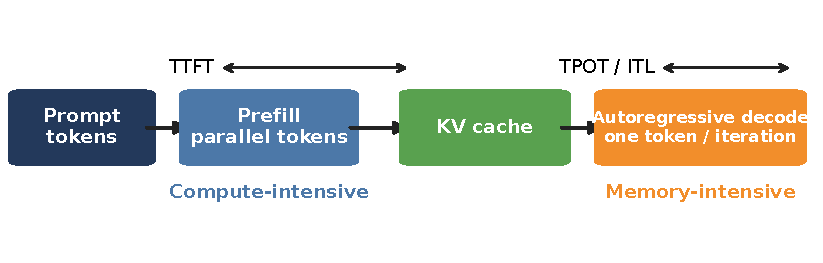
\includegraphics[width=\columnwidth]{figure/llm_inference_pipeline.pdf}
  \caption{The prefill and autoregressive decode phases of LLM inference.}
  \label{fig:inference-pipeline}
\end{figure}

\subsection{Parallel Deployment of LLMs}
\label{sec:parallelism-background}

Large models and high request rates require multiple GPUs. Figure~\ref{fig:parallelism} illustrates the three parallel dimensions considered in this work~\cite{shoeybi2019megatron,rajbhandari2022deepspeedmoe,zhang2026distributedenergy,wu2024loongserve,su2025seesaw}. Data parallelism (DP) replicates the model and partitions requests among replicas, increasing aggregate throughput at the cost of replicated weights. Tensor parallelism (TP) shards tensors or operators across GPUs and uses collectives to combine partial results; it reduces per-GPU memory demand but adds communication to each layer. Expert parallelism (EP) distributes MoE experts across GPUs and uses token dispatch and combine communication around routed FFN computation. Real deployments often combine DP, TP, and EP. Their compute utilization, memory footprint, and communication volume differ, so the fastest or lowest-power plan is not necessarily the most energy-efficient one.

\begin{figure}[t]
  \centering
  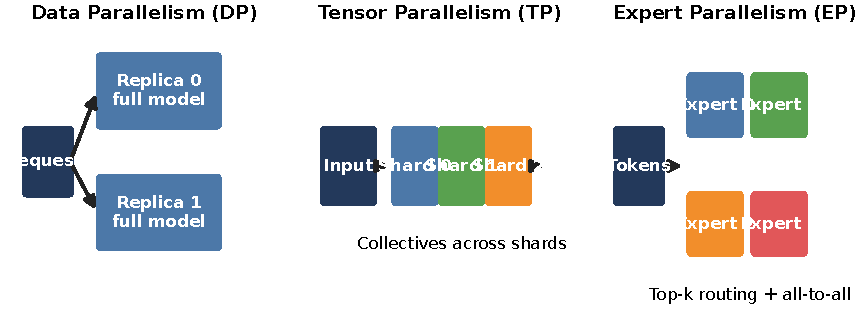
\includegraphics[width=\columnwidth]{figure/parallelism_dp_tp_ep.pdf}
  \caption{DP replicates models, TP shards operators, and EP distributes routed experts.}
  \label{fig:parallelism}
\end{figure}

\subsection{Disaggregated Serving Architectures}
\label{sec:disaggregation-background}

A conventional Native deployment executes prefill, decode, attention, and FFN computation in the same worker group. Prior systems introduced PD for phase-specialized serving and AF for disaggregated expert execution~\cite{zhong2024distserve,zhu2025megascale,patel2024splitwise,strati2024dejavu,lin2024infinitellm}. Disaggregation separates components with different resource characteristics so that they can be provisioned and scaled independently (Figure~\ref{fig:architectures}). Prefill--decode disaggregation (PD) assigns the two inference phases to separate pools and transfers request state and KV data from prefill workers to decode workers. Attention--FFN disaggregation (AF) separates the attention/KV path from dense or expert FFN computation and exchanges activations at transformer-layer boundaries. PD can match compute-oriented prefill with memory-oriented decode resources, while AF can specialize resources for attention and FFN. Both, however, introduce communication, synchronization, and pipeline overhead; whether separation saves energy depends on workload shape, parallel placement, and the underlying interconnect.

\begin{figure}[t]
  \centering
  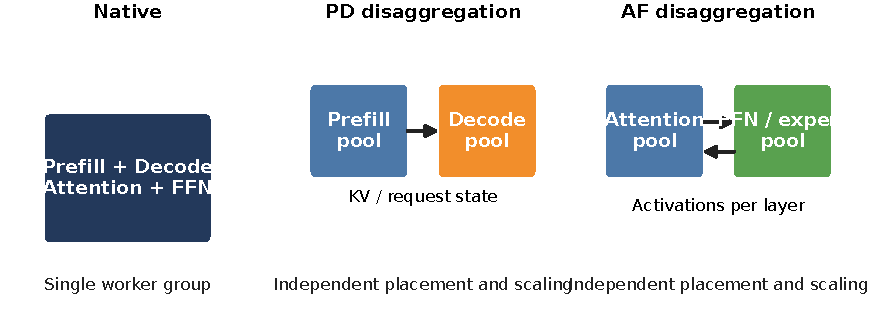
\includegraphics[width=\columnwidth]{figure/serving_architectures.pdf}
  \caption{Native, prefill--decode (PD), and attention--FFN (AF) serving architectures.}
  \label{fig:architectures}
\end{figure}

\subsection{Energy Management for LLM Serving}
\label{sec:energy-background}

Energy is the integral of power over execution time. A lower power draw therefore does not guarantee lower energy if it also extends request processing. Modern GPUs expose several control mechanisms, including core and memory dynamic voltage and frequency scaling (DVFS), power caps, and device consolidation~\cite{stojkovic2025dynamollm,kakolyris2025throttll,basit2026biscale,wang2025using,chung2025mlenergy}. Serving systems additionally control batching, placement, parallelism, and replica count. As shown in Figure~\ref{fig:energy-management}, an energy manager observes workload and system state, selects hardware and serving controls, and receives feedback through latency, throughput, power, and energy measurements. Useful policies must preserve TTFT/TPOT objectives while minimizing joules per request or maximizing tokens per joule. The best setting is architecture dependent because Native, PD, and AF expose different compute slack, memory traffic, and communication stalls.

\begin{figure}[t]
  \centering
  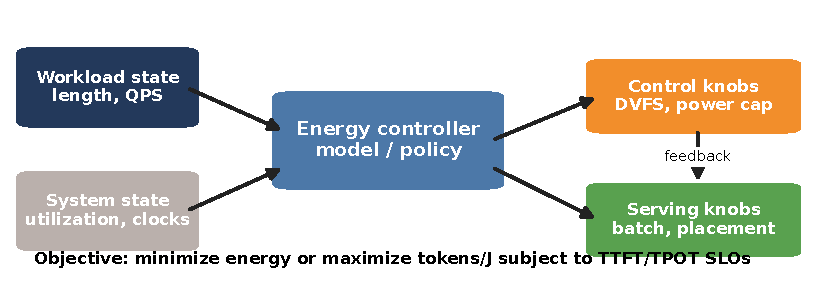
\includegraphics[width=\columnwidth]{figure/energy_management_loop.pdf}
  \caption{Closed-loop energy management for SLO-constrained LLM serving.}
  \label{fig:energy-management}
\end{figure}

\subsection{Datacenter and Consumer GPUs}
\label{sec:gpu-background}

GPUs used for LLM inference broadly fall into datacenter and consumer classes. Datacenter GPUs are designed for sustained multi-user operation and typically emphasize large error-correcting memory, predictable thermal behavior, remote manageability, virtualization, and high-speed scale-up or scale-out communication. Depending on the product family, they may provide NVLink/NVSwitch, GPUDirect RDMA, Multi-Instance GPU support, and stable power or clock controls. These features make datacenter GPUs suitable for multi-GPU serving and for deployments in which communication, availability, and isolation are first-order concerns~\cite{nvidiaA800datasheet,nvidiaL40Sspec,nvidiaL20spec}.

Consumer GPUs target interactive graphics and workstation workloads. They can offer high arithmetic throughput and favorable acquisition cost, but generally provide less memory, lack datacenter features such as NVLink and MIG, and have different cooling, reliability, and management assumptions. For example, the RTX~5090 exposes high Tensor throughput and fast GDDR7 memory but is a PCIe device without NVLink~\cite{nvidiaRTXBlackwell}. Consequently, peak FLOPS alone do not determine suitability for LLM serving: model capacity, memory behavior, communication requirements, power limits, and operational constraints all affect performance and energy efficiency. This distinction motivates evaluating both datacenter and consumer GPU classes rather than extrapolating conclusions from a single platform.


\section{Related Work}

\noindent{\textbf{LLM serving and resource management.}}
Modern serving systems improve throughput and latency through iteration-level scheduling, continuous or hybrid batching, request migration, and SLO-aware resource allocation~\cite{yu2022orca,kwon2023vllm,agrawal2024sarathi,sun2024llumnix,duan2024muxserve,hong2025sola}. Constraint-aware schedulers select batch sizes and parallel configurations from workload distributions, while simulation frameworks use operator profiles to explore large deployment spaces~\cite{agrawal2024vidur}. Recent systems further adapt model sharding across prefill and decode or optimize placement over heterogeneous GPUs and networks~\cite{su2025seesaw,jiang2025thunderserve,mei2025helix}. These systems primarily optimize goodput, latency, utilization, or monetary cost; energy is rarely the principal comparison boundary.

\noindent{\textbf{Disaggregated inference.}}
P/D systems isolate compute-intensive prefill from memory-intensive decode so that each phase can use an independent parallel plan and resource pool. DistServe co-optimizes phase placement and goodput under TTFT/TPOT objectives, while Splitwise studies homogeneous and heterogeneous phase-specific clusters~\cite{zhong2024distserve,patel2024splitwise}. DejaVu streams KV state to support disaggregation and fault tolerance, and Mooncake builds a KVCache-centric transfer and storage substrate~\cite{strati2024dejavu,qin2024mooncake}. Other systems combine disaggregation with chunked prefill, dynamic re-sharding, or data-reduced orchestration to reduce phase interference and transfer pressure~\cite{su2025seesaw}. Beyond P/D, Infinite-LLM separates attention and non-attention execution for distributed long-context serving, MegaScale-Infer disaggregates attention and experts, and OPSCALE provisions individual operators~\cite{lin2024infinitellm,zhu2025megascale,cui2026opscale}. This literature establishes that the disaggregation boundary changes utilization and communication, but does not systematically compare the resulting energy behavior across Native, PD, and AF.

\noindent{\textbf{KV-cache and long-context optimization.}}
KV-cache work spans paging, compression, sparsity, offloading, streaming, and reuse. PagedAttention reduces fragmentation, RadixAttention reuses shared prefixes, Marconi manages prefix state for hybrid models, and CacheBlend selectively recomputes reusable caches for RAG contexts~\cite{kwon2023vllm,zheng2024sglang,pan2025marconi,yao2025cacheblend}. Quantization and selective-attention methods reduce cache bytes or accessed pages, while unified sparse attention addresses both long-prefill computation and decode KV traffic~\cite{zhang2023h2o,xiao2024streamingllm,li2024snapkv,chen2024arkvale,lin2025qserve,yang2025lserve,gao2025rethinkingkv}. Offloading systems prefetch selected KV entries from CPU memory or exploit memory elsewhere in a scale-up GPU domain~\cite{lee2024infinigen,kumar2025aqua}. CacheGen compresses KV state for network streaming, making it directly relevant to disaggregated transfer cost~\cite{liu2024cachegen}. Long-context systems additionally use elastic sequence parallelism and customizable attention kernels to balance computation, memory, and communication~\cite{wu2024loongserve,ye2025flashinfer}. These methods alter the amount and location of state moved by PD and AF, yet their deployment-level energy consequences remain underexplored.

\noindent{\textbf{Power management and energy-efficient serving.}}
A growing body of work coordinates runtime decisions with GPU power controls. DynamoLLM profiles model and request-class energy behavior, maintains differently configured instance pools, and uses hierarchical controllers to resize pools and select tensor-parallel and GPU-frequency configurations under latency SLOs~\cite{stojkovic2025dynamollm}. throttLL'eM predicts future batch and KV-cache states and selects an energy-efficient frequency and engine configuration~\cite{kakolyris2025throttll}. GreenLLM applies phase-aware frequency scaling, BiScale combines P/D placement with fine-grained DVFS, and PALS jointly controls GPU power caps and batch size for MoE serving~\cite{liu2025greenllm,basit2026biscale,hankendi2026pals}. AFlex combines P/D and A/F disaggregation into independently provisioned PA, PF, DA, and DF pools with operator--phase-specific frequency control~\cite{hu2026energy}. Fine-grained accelerator models and recent inference-energy benchmarks broaden the available control and measurement methodology~\cite{wang2025using,chung2025mlenergy}. These approaches optimize particular architectures or knobs; our goal is to characterize how the architecture itself changes the available energy trade-off.

\noindent{\textbf{Characterizing performance and energy.}}
Measurement work shows that power, runtime, and energy must be evaluated together. Distributed-training studies demonstrate that parallel configuration and GPU frequency interact through different computation--communication ratios~\cite{zhang2026distributedenergy}. For inference, recent studies characterize multi-request workflows, request- and token-level costs, and cross-model or cross-hardware behavior~\cite{ifath2026characterizing,vellaisamy2026characterization,chung2025mlenergy}. Hardware benchmarks likewise expose substantial performance variation across GPU and accelerator families~\cite{agrawal2024vidur}. However, these studies focus on training, monolithic inference, application workflows, or broad benchmark coverage. They do not isolate the energy impact of alternative disaggregation boundaries under matched workloads, networks, parallel plans, and GPU characteristics.

\noindent{\textbf{Comparison with existing work.}}
Table~\ref{tab:related-comparison} summarizes the scope of representative studies. Existing measurement work mainly considers monolithic inference or distributed training, whereas disaggregated-serving work primarily targets performance and resource efficiency. Energy-aware serving systems optimize a particular architecture or control mechanism. In contrast, our study uses a common measurement methodology to compare Native, PD, and AF serving across multiple GPU classes, interconnects, and parallel deployment paradigms.

\begin{table*}[t]
  \caption{Scope comparison with representative existing work. ``Energy'' denotes direct energy measurement or optimization.}
  \label{tab:related-comparison}
  \centering
  \small
  \setlength{\tabcolsep}{4pt}
  \begin{tabular}{lccccccc}
    \toprule
    Work & Energy & Native & PD & AF & Multiple GPU classes & Network effects & DP/TP/EP \\
    \midrule
    DistServe~\cite{zhong2024distserve} & -- & -- & Yes & -- & -- & -- & -- \\
    MegaScale-Infer~\cite{zhu2025megascale} & -- & -- & -- & Yes & Yes & Yes & Yes \\
    DynamoLLM~\cite{stojkovic2025dynamollm} & Yes & Yes & -- & -- & -- & -- & TP \\
    BiScale~\cite{basit2026biscale} & Yes & -- & Yes & -- & -- & Yes & -- \\
    throttLL'eM~\cite{kakolyris2025throttll} & Yes & Yes & -- & -- & Yes & -- & TP \\
    Req-Token Energy~\cite{vellaisamy2026characterization} & Yes & Yes & -- & -- & Yes & -- & -- \\
    Zhang et al.~\cite{zhang2026distributedenergy} & Yes & -- & -- & -- & Yes & Yes & Yes \\
    \textbf{This work} & Yes & Yes & Yes & Yes & Yes & Yes & Yes \\
    \bottomrule
  \end{tabular}
\end{table*}



\section{Experimental Setup and Methodology}
\label{sec:methodology}

This section describes the experimental platforms, workloads, deployment configurations, and measurement methodology. The individual experiments and research questions are presented in Section~5.

\subsection{Hardware Configuration}
\label{sec:hardware}

Our hardware matrix covers both datacenter and consumer GPUs with different compute throughput, memory capacity, memory technology, and interconnect support. Table~\ref{tab:hardware} summarizes the principal devices. NVIDIA A800-SXM4-80GB servers form the primary datacenter platform. Each server contains eight GPUs connected by NVLink/NVSwitch; PCIe and GPUDirect RDMA are used for intra-host and inter-host communication experiments, respectively. L40S provides a datacenter comparison with higher arithmetic throughput but lower memory capacity and bandwidth. RTX~5090 is the consumer-GPU platform, while L20 is a PCIe datacenter GPU. Both use GDDR memory and lack NVLink, complementing the tightly coupled A800 SXM platform.

\begin{table}[t]
  \caption{Principal GPU platforms. Compute values are dense peak TFLOPS without structured sparsity.}
  \label{tab:hardware}
  \centering
  \small
  \setlength{\tabcolsep}{2.5pt}
  \resizebox{\columnwidth}{!}{%
  \begin{tabular}{lrrrll}
    \toprule
    GPU & FP32 & FP16/BF16 & Memory & Bandwidth & Class \\
    \midrule
    A800 SXM4 & 19.5 & 312   & 80 GB HBM2e & 2039 GB/s & Datacenter \\
    L40S      & 91.6 & 362   & 48 GB GDDR6 & 864 GB/s  & Datacenter \\
    RTX 5090  & 104.8 & 419  & 32 GB GDDR7 & 1792 GB/s & Consumer \\
    L20       & 59.3 & 119.5 & 48 GB GDDR6 & 864 GB/s  & Datacenter \\
    \bottomrule
  \end{tabular}}
\end{table}

To isolate network effects, only the A800 platform is used for the network comparison. A800 deployments exercise NVLink/NVSwitch within a server, PCIe-isolated placements, and GPUDirect RDMA across two or four servers while preserving the intended GPU budget. L40S, RTX~5090, and L20 are not included in the network-variable experiment; they use their platform-local PCIe connectivity. Every run records the GPU model and UUID, participating devices, GPU--NIC affinity, applied clock state, and observed transport so that an unintended communication path cannot be mistaken for the target topology.

Host CPUs launch workers, route requests, and coordinate measurements, but CPU type and CPU parallelism are not experimental variables. Paired comparisons use the same host allocation and process placement. Because the current energy scope is the set of GPUs assigned to a deployment, CPU and network-device energy are not included in the reported joules; this boundary is stated explicitly when interpreting cluster-level energy results.

\subsection{Models, Workloads, and Parallelism}
\label{sec:models-workloads}

We select dense and mixture-of-experts (MoE) models at three scales (Table~\ref{tab:models}). For dense models, Small denotes fewer than 10 billion parameters, Middle denotes 10--50 billion, and Large denotes more than 50 billion. MoE systems have substantially different total and active parameter counts, so we use deployment-oriented tiers rather than forcing dense-model thresholds onto them: OLMoE-1B-7B represents Small, Qwen3-30B-A3B represents Middle, and Mixtral-8$\times$7B represents Large. Total parameters capture memory and placement cost, whereas active parameters approximate per-token expert computation.



\begin{table*}[t]
  \centering
  \begin{minipage}[t]{0.42\textwidth}
    \caption{Models included in the measurement matrix.}
    \label{tab:models}
    \centering
    \small
    \begin{tabular}{lll}
      \toprule
      Scale & Dense & MoE \\
      \midrule
      Small  & Llama-3.1-8B & OLMoE-1B-7B \\
      Middle & Qwen3-32B & Qwen3-30B-A3B \\
      Large  & Llama-3.3-70B & Mixtral-8$\times$7B \\
      \bottomrule
    \end{tabular}
  \end{minipage}
  \hfill
  \begin{minipage}[t]{0.54\textwidth}
    \caption{Fixed-shape workloads; lengths are in tokens.}
    \label{tab:workloads}
    \centering
    \small
    \begin{tabular}{lrrl}
      \toprule
      Workload & Input & Output & Regime \\
      \midrule
      QA          & 128   & 64   & LPLD \\
      Chatbot     & 128   & 1024 & LPHD \\
      Balanced    & 512   & 256  & MPMD \\
      RAG         & 4096  & 64   & HPLD \\
      Summary     & 4096  & 1024 & HPHD \\
      LongContext & 16384 & 256  & Long context \\
      \bottomrule
    \end{tabular}
  \end{minipage}
\end{table*}

The workload suite contains six fixed input/output shapes (Table~\ref{tab:workloads}). QA represents short-prefill/short-decode traffic, Chatbot is decode-heavy, Balanced has moderate input and output lengths, RAG is prefill-heavy, Summary combines a long prompt with a long response, and LongContext stresses long-prefill execution and KV-cache capacity. Requests are generated once from fixed seeds and replayed across configurations. An open-loop generator issues requests according to a Poisson process, preventing server response time from altering the offered arrival rate.



We support data parallelism (DP), tensor parallelism (TP), expert parallelism (EP), and their hybrid combinations. DP creates complete model replicas and distributes requests among them. TP shards dense operators across GPUs and introduces collective communication. EP distributes MoE experts and routes tokens to their selected experts. A deployment manifest records the DP, TP, and EP degree independently for every role. Unless parallelism itself is varied, a configuration uses the same total GPU budget as its architectural counterparts.

\subsection{Serving Architectures}
\label{sec:architectures}

We implement three serving architectures in SGLang. \emph{Native} is the non-disaggregated baseline: one worker group executes the complete model and colocates prefill and decode as well as attention and FFN computation. Its default eight-GPU configuration is TP8.

\emph{PD} separates prefill and decode into independent worker groups. The prefill group computes the prompt and transfers the resulting request state and KV cache to the decode group. Its default eight-GPU configuration assigns four GPUs to each group, denoted P-TP4 + D-TP4. The groups can also be placed on separate hosts to exercise RDMA communication.

\emph{AF} separates attention and FFN execution. Attention workers maintain the attention/KV path, while FFN workers execute dense or routed-expert computation; intermediate activations cross the pool boundary at transformer-layer granularity. Its default eight-GPU configuration is A-TP4 + F-TP4. AF can use NVLink within a host or RDMA across hosts, and each pool can independently use DP, TP, or EP.

All comparisons hold model precision, serving software, request stream, and total GPU allocation constant unless the evaluated configuration explicitly changes one of them. Prefix reuse is disabled to prevent cache-hit variation from confounding architecture comparisons. The complete deployment, rather than an individual worker or pool, is the unit of performance and energy accounting.

\subsection{Measurement Methodology and Metrics}
\label{sec:metrics}

Each configuration is launched as a fresh deployment and must pass readiness and health checks before measurement. After any required warm-up, the load generator replays the frozen request stream and waits for all admitted requests to complete or time out. Configurations are executed serially to avoid resource interference, and each reported point uses three independent repetitions. The deployment manifest and system snapshots preserve model, placement, topology, process, and clock information needed to reproduce a run.

We obtain GPU energy from NVML cumulative-energy counters and calculate consumed energy from counter differences over the same interval used for request measurement. Cluster GPU energy is the sum over only the GPUs assigned in the deployment plan, and average GPU power is total GPU energy divided by measurement duration. Per-GPU and per-node values are retained to reveal role or placement imbalance. On devices or clock domains that do not expose a reliable cumulative counter, the applicable telemetry source and integration method are recorded with the result.

Performance metrics include offered and achieved QPS, input- and output-token throughput, end-to-end latency, time to first token (TTFT), time per output token (TPOT), and inter-token latency (ITL). We report mean and p50/p90/p95/p99 latency where applicable. Energy-efficiency metrics include total joules, average power, joules per successful request, joules per input token, joules per output token, joules per total token, and input/output/total tokens per joule. Network configurations additionally record link validation and telemetry; system snapshots include GPU utilization, memory use, temperature, and core/memory clocks.

A run is valid only when the deployment remains healthy, at least 99\% of requests succeed, and the load generator reproduces the configured open-loop arrival process. We compare energy efficiency only among configurations satisfying the same service-level objective and having all three repetitions. This joint treatment of runtime, power, and energy is necessary because reducing instantaneous power can increase execution time and therefore fail to reduce total energy~\cite{zhang2026distributedenergy}.


\section{Results}

This section presents the evaluation results by answering the following research questions.

\noindent{RQ1:Which dataset is more energy efficient for which deployment architecture?}

\noindent{RQ2:Which communication efficiency is more beneficial to which discrete architectures?}

\noindent{RQ3:How different parallel deployment paradigms affect different decoupling architectures?}

\noindent{RQ4:Which compute-memory ratio offers the best prospects for energy efficiency in which discrete architecture?}

\noindent{RQ5:Investigating the impact of HBM frequency tuning on different discrete architectures?}

\subsection{RQ1}

\subsection{RQ2}

\subsection{RQ3}

\subsection{RQ4}

\subsection{RQ5}

\section{Discussion}
\label{sec:discussion}

\subsection{Interpreting Performance--Energy Trade-offs}
\label{sec:discussion-tradeoffs}

The energy efficiency of an LLM serving architecture is determined jointly by average power and execution time. A deployment that lowers GPU utilization or operating frequency may draw less power but consume more total energy if communication, synchronization, or slower computation substantially extends the measurement interval. Conversely, a high-power configuration can be energy efficient when it completes requests quickly and returns accelerators to an idle or reusable state. Therefore, architecture comparisons should not rank systems by power, latency, or throughput in isolation. We interpret a configuration as preferable only when it satisfies the same service-level objective (SLO) and improves normalized energy metrics such as joules per successful request or tokens per joule.

This distinction is particularly important for disaggregated serving. PD and AF can specialize worker pools for phases or operators with different resource demands, but they also introduce data movement and coordination. The relevant question is not whether disaggregation reduces the power of an individual pool, but whether the reduction in computation or interference outweighs transfer energy, synchronization delay, pipeline bubbles, and the baseline power of additional active GPUs. Reporting per-role energy alongside deployment-level energy helps identify whether an apparent gain comes from genuine efficiency or from shifting work to another pool.

\subsection{Implications for Deployment Design}
\label{sec:discussion-implications}

No serving architecture should be expected to dominate across all workloads and platforms. Prefill-heavy workloads expose more compute parallelism, whereas decode-heavy and long-context workloads place greater pressure on model and KV-cache bandwidth. Native serving avoids inter-pool transfers but couples components with different scaling behavior. PD can independently provision compute-oriented prefill and memory-oriented decode, while AF can specialize attention and FFN resources, particularly for MoE models. The preferred architecture can consequently change with the input/output ratio, offered load, model type, and SLO.

Communication and parallelism must be considered as part of the architecture rather than as independent implementation details. TP and EP add frequent collectives or token exchange; PD transfers request state and KV data; and AF exchanges activations at layer boundaries. Fast scale-up links can hide or amortize some of these costs, whereas PCIe or multi-node RDMA may move the energy--performance crossover. Similarly, increasing DP can raise throughput through replication but also duplicates model memory and idle power. Practical provisioning should therefore select the architecture, role placement, and DP/TP/EP degrees jointly.

Hardware selection creates another trade-off. Datacenter GPUs provide large ECC memory and high-speed interconnects, while consumer GPUs can provide high arithmetic throughput at different capacity, management, and connectivity points. Peak FP16/BF16 throughput alone does not predict serving efficiency: decode can remain memory-bound, a model may not fit at the desired parallel degree, and a disaggregated design may depend more on communication than arithmetic capability. Frequency controls should likewise be applied selectively. Compute-bound components are more sensitive to core-frequency reductions, whereas memory- or communication-stalled components may tolerate them. Memory-frequency reductions are useful only when their power savings exceed the additional service time and do not violate the SLO.

\subsection{Measurement Scope and Threats to Validity}
\label{sec:discussion-validity}

Our conclusions are bounded by the evaluated models, request shapes, hardware, software version, and deployment configurations. The fixed-shape workloads isolate input/output effects and improve repeatability, but production traffic includes correlations, multi-turn context, shared prefixes, burstiness, cancellations, and changing output distributions. Open-loop Poisson arrivals do not reproduce every production process. Results should therefore be interpreted as controlled architectural characterization rather than a complete model of every deployment.

Hardware and software effects also limit generalization. GPU firmware, drivers, kernels, quantization, attention backends, routing policies, and batching algorithms can change utilization and energy. Product-level peak specifications do not guarantee realized throughput. We mitigate these effects by keeping the software and precision fixed within paired comparisons, recording manifests and system state, validating communication paths, and repeating deployments; nevertheless, results from the evaluated GPUs should not be directly extrapolated to accelerators with different memory hierarchies or interconnects.

The energy boundary is another limitation. Our primary metric includes the GPUs assigned to a deployment because their cumulative energy counters provide a consistent measurement across configurations. It does not include host CPU, DRAM, NIC, switch, storage, cooling, or power-conversion losses. This boundary is suitable for comparing GPU execution but can understate the cost of multi-node and communication-intensive architectures. Future work should combine device counters with node- and rack-level metering and should account for embodied carbon and regional electricity carbon intensity.

Finally, SLO filtering can introduce survivorship bias if only successful high-load configurations remain. We therefore report offered and achieved load, success rate, and latency distributions and compare energy only among configurations satisfying the same validity criteria. Repeated trials quantify run-to-run variation, but longer-duration studies are still needed to capture thermal drift, failures, autoscaling transients, and diurnal workloads.

\subsection{Toward Architecture-Aware Energy Management}
\label{sec:discussion-future}

The measurement dimensions in this study suggest that energy management should be architecture aware. Rather than tuning frequency, batch size, parallelism, or placement independently, a controller could use workload composition and measured phase/operator sensitivity to choose a complete operating point. Such a controller would select among Native, PD, and AF; assign hardware to each role; determine DP/TP/EP degrees; and apply role-specific core or memory settings subject to TTFT, TPOT, capacity, and power constraints. The resulting objective is a constrained Pareto optimization problem rather than simple power minimization.

A useful next step is to construct predictive models from the collected measurements. These models should capture computation, memory traffic, communication, synchronization, and idle power separately and estimate both latency and energy before deployment. Online feedback could then correct prediction error and adapt to workload drift. Extending the methodology to multi-tenant serving, heterogeneous accelerators, shared KV-cache tiers, node-level energy measurement, and carbon-aware placement would provide a more complete foundation for sustainable LLM infrastructure.


\section{Conclusion}
\label{sec:conclusion}

This paper establishes a systematic methodology for understanding the performance and GPU-energy behavior of non-disaggregated and disaggregated LLM serving. We compare Native, prefill--decode (PD), and attention--FFN (AF) architectures in a common SGLang implementation under matched models, request streams, SLOs, and accelerator budgets. The study spans dense and MoE models, diverse input/output regimes, DP/TP/EP and hybrid parallelism, datacenter and consumer GPUs, NVLink/PCIe/RDMA communication, compute--memory capability, and GPU operating settings. By measuring latency, throughput, power, and total energy over the same request interval, the methodology avoids treating lower power as synonymous with greater energy efficiency.

The central premise of this work is that serving architecture cannot be evaluated independently of workload, placement, communication, and hardware. Disaggregation offers specialization and independent scaling, but its benefits must offset state transfer, activation communication, synchronization, and additional device residency. Likewise, a throughput-optimal parallel plan or a lower-frequency operating point is not necessarily energy optimal. Reproducible deployment manifests, communication validation, SLO-aware filtering, per-GPU energy accounting, and repeated open-loop trials provide the evidence needed to identify these trade-offs.

Our characterization is intended to support both system designers and operators: it provides a common basis for selecting architectures and deployment configurations and motivates future controllers that jointly optimize architecture, parallelism, placement, and frequency. As LLM inference becomes a growing component of datacenter electricity demand, such architecture-aware performance--energy analysis will be essential for building scalable and sustainable serving systems.


\begin{acks}
To Robert, for the bagels and explaining CMYK and color spaces.
\end{acks}

\bibliographystyle{ACM-Reference-Format}
\bibliography{sections/reference}

\end{document}